\documentclass{article}
\usepackage{graphicx} % Required for inserting images
\usepackage[utf8]{inputenc}
\usepackage{polski}
\usepackage[dvipsnames]{xcolor}
\usepackage{indentfirst}
\usepackage{multicol}
\usepackage{geometry}
\usepackage{titlesec}
\usepackage[colorlinks=true, linkcolor=gray, urlcolor=blue, citecolor=green]{hyperref}
\usepackage{makecell}
\usepackage{float}
\usepackage[polish]{babel}
\usepackage[T1]{fontenc}
\usepackage[justification=centering]{caption}
\usepackage[utf8]{inputenc} 
\usepackage{subfig}
\usepackage{changepage}


\usepackage{mwe} % for 'example-image'
\usepackage{newfloat}
\DeclareFloatingEnvironment{graph}
\addto\captionspolish{%
  \renewcommand{\graphname}{Wykres}%
  \renewcommand{\figurename}{Zdjęcie}%
  \renewcommand{\tablename}{Tabela}%
}


\begin{document}

\begin{titlepage}
    \begin{center}
        \vspace*{1cm}
            
        \Huge
        \textbf{Sprawozdanie z laboratorium 1}
            
        \vspace{0.5cm}
        \LARGE
        Podstawy PLC (IDEC)
            
        \vspace{1.5cm}
            
        \textbf{Łukasz Janusz\\Marek Generowicz}

        \normalsize      
        \textcolor{gray}{10.04.2025}
        \vfill
        \begin{figure}[hb]
            \centering
            
\includegraphics[width=0.5\textwidth]{media/Logo_AGH.jpg}
        \end{figure}   
    \end{center}
\end{titlepage}

\newpage
\section{Wstęp}
Na zajęciach należało zaprogramować sterownik FC6A marki IDEC. Wykonano to w środowisku WindLDR V8.

Sterownik znajdował się w skrzynce sterowniczej, która była podłączona do komputera. W skrzynce znajdowały się dwa moduły rozszerzeń, które były podłączone do sterownika. Użytkownik miał możliwość kontrolowania 6 wyjść analogowych oraz panelu sterowniczego, jednak na zajęciach należało się skupić tylko na części z nich. Wnętrze skrzynki sterowniczej przedstawia zdjęcie \ref{fig:zdj2}.

Stanowisko składało się z kaskadowego układu zbiorników bezciśnieniowych. Ruch cieczy do zbiorników wyżej położonych umożliwiał silnik elektryczny, zasilany falownikiem umożliwiającym regulacje prędkości silnika. W dół ciecz spływała grawitacyjnie. Połączenia między zbiornikami były kontrolowane za pomocą zaworów kulkowych lub za pomocą zaworów regulacyjnych z pozycjonerami z elektrycznymi siłownikami silnikowymi. Cały układ przedstawia zdjęcie \ref{fig:zdj1}. 


\begin{figure}[H]
    \centering
        % Pod figura 1
        \subfloat[Skrzynka sterownicza (zdjęcie z konspektu)]{    
            \centering
            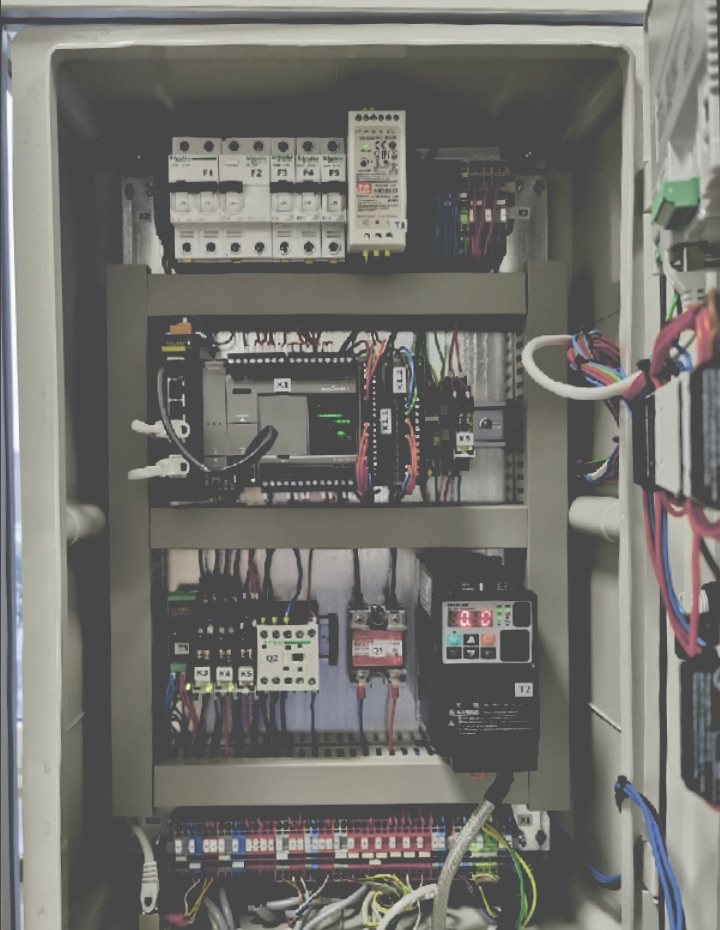
\includegraphics[width=0.45\textwidth]{media/0_Wnetrze_skrzynki.jpeg}
            \label{fig:zdj2}}
        % Pod figura 1
        \subfloat[Całe stanowisko (zdjęcie z konspektu)]{
            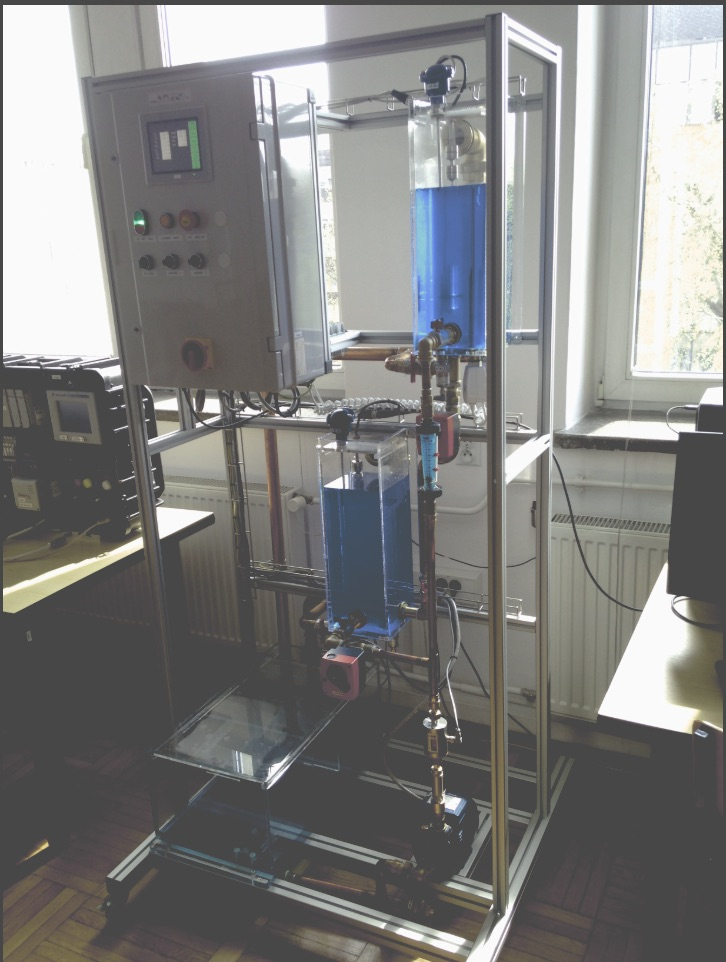
\includegraphics[width=0.45\textwidth]{media/0_Całe_stanowisko(Z konspektu).jpeg}
            \label{fig:zdj1}}
    \caption{Skrzynka sterownicza oraz stanowisko (zdjęcia z konspektu)}
    \label{fig:main0}
\end{figure}


\newpage
\section{Konfiguracja sterownika}
Przed przystąpieniem do programowania sterownika, należało skonfigurować parametry komunikacji. 

Na zdjęciu \ref{fig:zdj3} pokazane są parametry, które należało ustawić jako parametry sieci w PLC, aby ten mógł poprawnie połączyć się z fizycznym sterownikiem.

\begin{figure}[H]
    \centering
    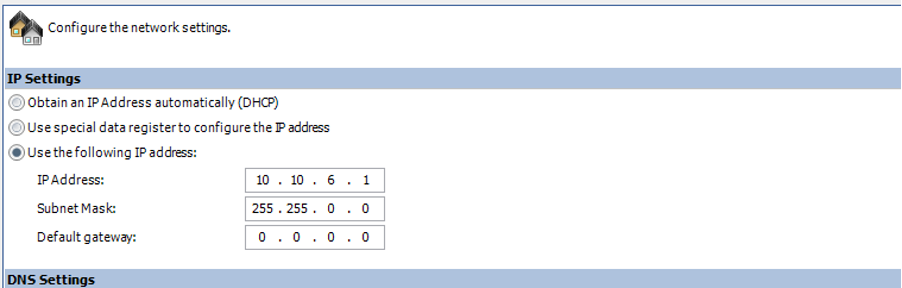
\includegraphics[width=0.5\textwidth]{media/1_1_Network_setting.png}
    \caption{Konfiguracja sieci dla sterownika}
    \label{fig:zdj3}
\end{figure}


Następnie skonfigurowano ustawienia komunikacji programu. W tym celu należało ustawić komunikacje przez \textit{Ethernet} oraz ustawić odpowiednie parametry. Na zdjęciu \ref{fig:zdj4} pokazano jakie dokładnie wartości należało ustawić.
\begin{figure}[H]
    \centering
    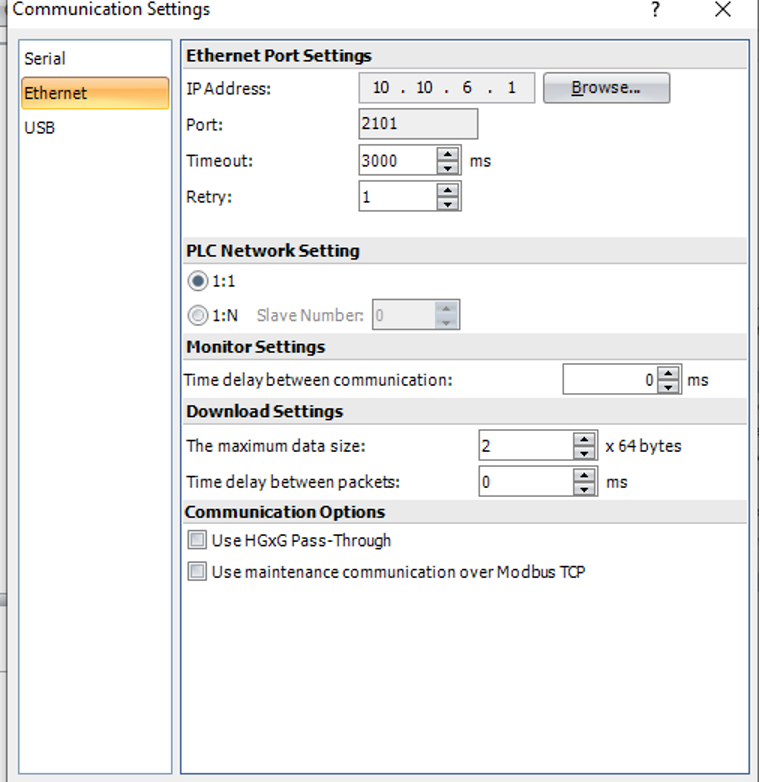
\includegraphics[width=0.5\textwidth]{media/1_2_Coms_setting.png}
    \caption{Konfiguracja komunikacji programu}
    \label{fig:zdj4}
\end{figure}

\newpage
Po skonfigurowaniu połączenia możliwe jest automatyczne podpięcie modułów wejść oraz wyjść w aplikacji. Dzięki temu do układu zostały podpięte dwa moduły analogowe, które następnie należało skonfigurować zgodnie z dokumentacją stanowiska, moduł pierwszy, zgodnie z zdjęciem \ref{fig:zdj5} odpowiada za wejścia, a moduł drugi, zgodnie z zdjęciem \ref{fig:zdj6} odpowiada za wyjścia. Dzięki takiej konfiguracji możliwe jest podpięcie odczyt oraz kontrola zmiennych procesowych. 

\begin{figure}[H]
    \centering
        % Pod figura 1
        \subfloat[Moduł I]{    
            \centering
            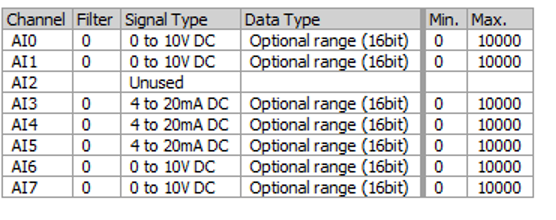
\includegraphics[width=0.45\textwidth]{media/1_3_Mod1_tags.png}
            \label{fig:zdj5}}
        % Pod figura 1
        \subfloat[Moduł II]{
            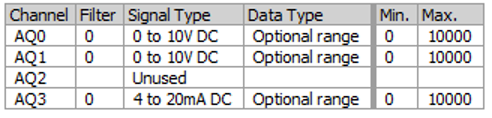
\includegraphics[width=0.45\textwidth]{media/1_4_Mod2_tags.png}
            \label{fig:zdj6}}
    \caption{Konfiguracja rejestrów dla modułów}
    \label{fig:main1}
\end{figure}

Po podpięciu modułów, możliwe jest odczytanie ich wartości. W tym celu należało uruchomić opcje \textit{Monitor}  w zakładce \textit{Module Configuration}. Dzięki temu możliwe jest odczytanie wartości wejść, które są podpięte do modułu 1. Zdjęcie \ref{fig:zdj7} przedstawia jak wygląda moduł 1 po połączeniu z sterownikiem.

Ważne aby pamiętać że wyniki wejść nie są w jednostkach fizycznych, a w jednostkach cyfrowych. W celu przeliczenia ich na jednostki fizyczne, w tym celu należy podzielić podaną wartość przez 100 lub dla przepływu przez 400.


\begin{figure}[H]
    \centering
    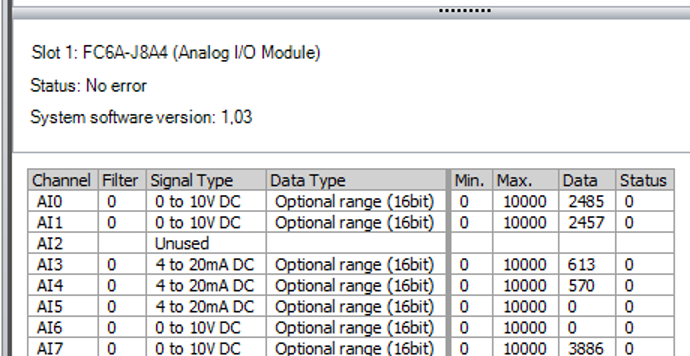
\includegraphics[width=0.5\textwidth]{media/1_5_Odczyt_zmiennych.png}
    \caption{Wartości zmiennych w module 1}
    \label{fig:zdj7}
\end{figure}

\newpage
Alternatywnie można użyć opcji \textit{Batch Monitor}, która pozwala na odczytanie które z zmiennych procesowych są używane w danym momencie. Zdjęcie \ref{fig:zdj8} przedstawia jak wygląda opcja \textit{Batch Monitor}. 

Warto zauważyć że do dyspozycji w wierszu pierwszym mamy 14 komórek. W przypadku naszego sterownika mamy do dyspozycji 14 wejść więc w przypadku odczytu wejść jedynie przydatny pierwszy wiersz tabeli.
\begin{figure}[H]
    \centering
    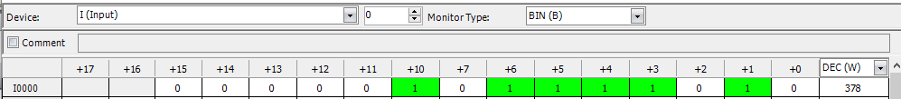
\includegraphics[width=0.5\textwidth]{media/1_6_Batch_monitor.png}
    \caption{Batch monitor}
    \label{fig:zdj8}
\end{figure}

\newpage
\section{Zmienne procesowe}
Po skonfigurowaniu sterownika oraz podpięciu modułów, należało przestąpić do programowania sterownika tak aby można było go kontrolować. 

W pierwszej kolejności należało stworzyć drabinkę pozwalającą włączać oraz resetować przekaźnik \textit{K4}, który jest przypisany do zmiennej \textit{Q6}. Aby to zrobić, warto było stworzyć tagi rejestrów nazywającym się \textit{START} oraz \textit{STOP}. Następnie tak przypisane tagi należało odpowiednio podpiąć do zmiennej \textit{Q6}. Program powinien wyglądać jak na zdjęciu \ref{fig:zdj9}.

\begin{figure}[H]
    \centering
    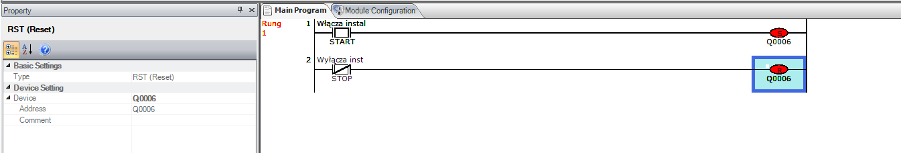
\includegraphics[width=0.5\textwidth]{media/2_1_Podstawowe_bramki_do_guzikow.png}
    \caption{Program do włączania oraz resetowania przekaźnika}
    \label{fig:zdj9}
\end{figure}

Następnie należało dodać drabinkę dzięki której wraz z zmianą wartości zmiennej \textit{Q6} zmienia zapala się zielona lampka jak na zdjęciu \ref{fig:zdj10}. W tym celu należało ustawić że wartość zmiennej \textit{Q4} zmienia się wraz z zmianą wartości zmiennej \textit{Q6}. 

\begin{figure}[H]
    \centering
    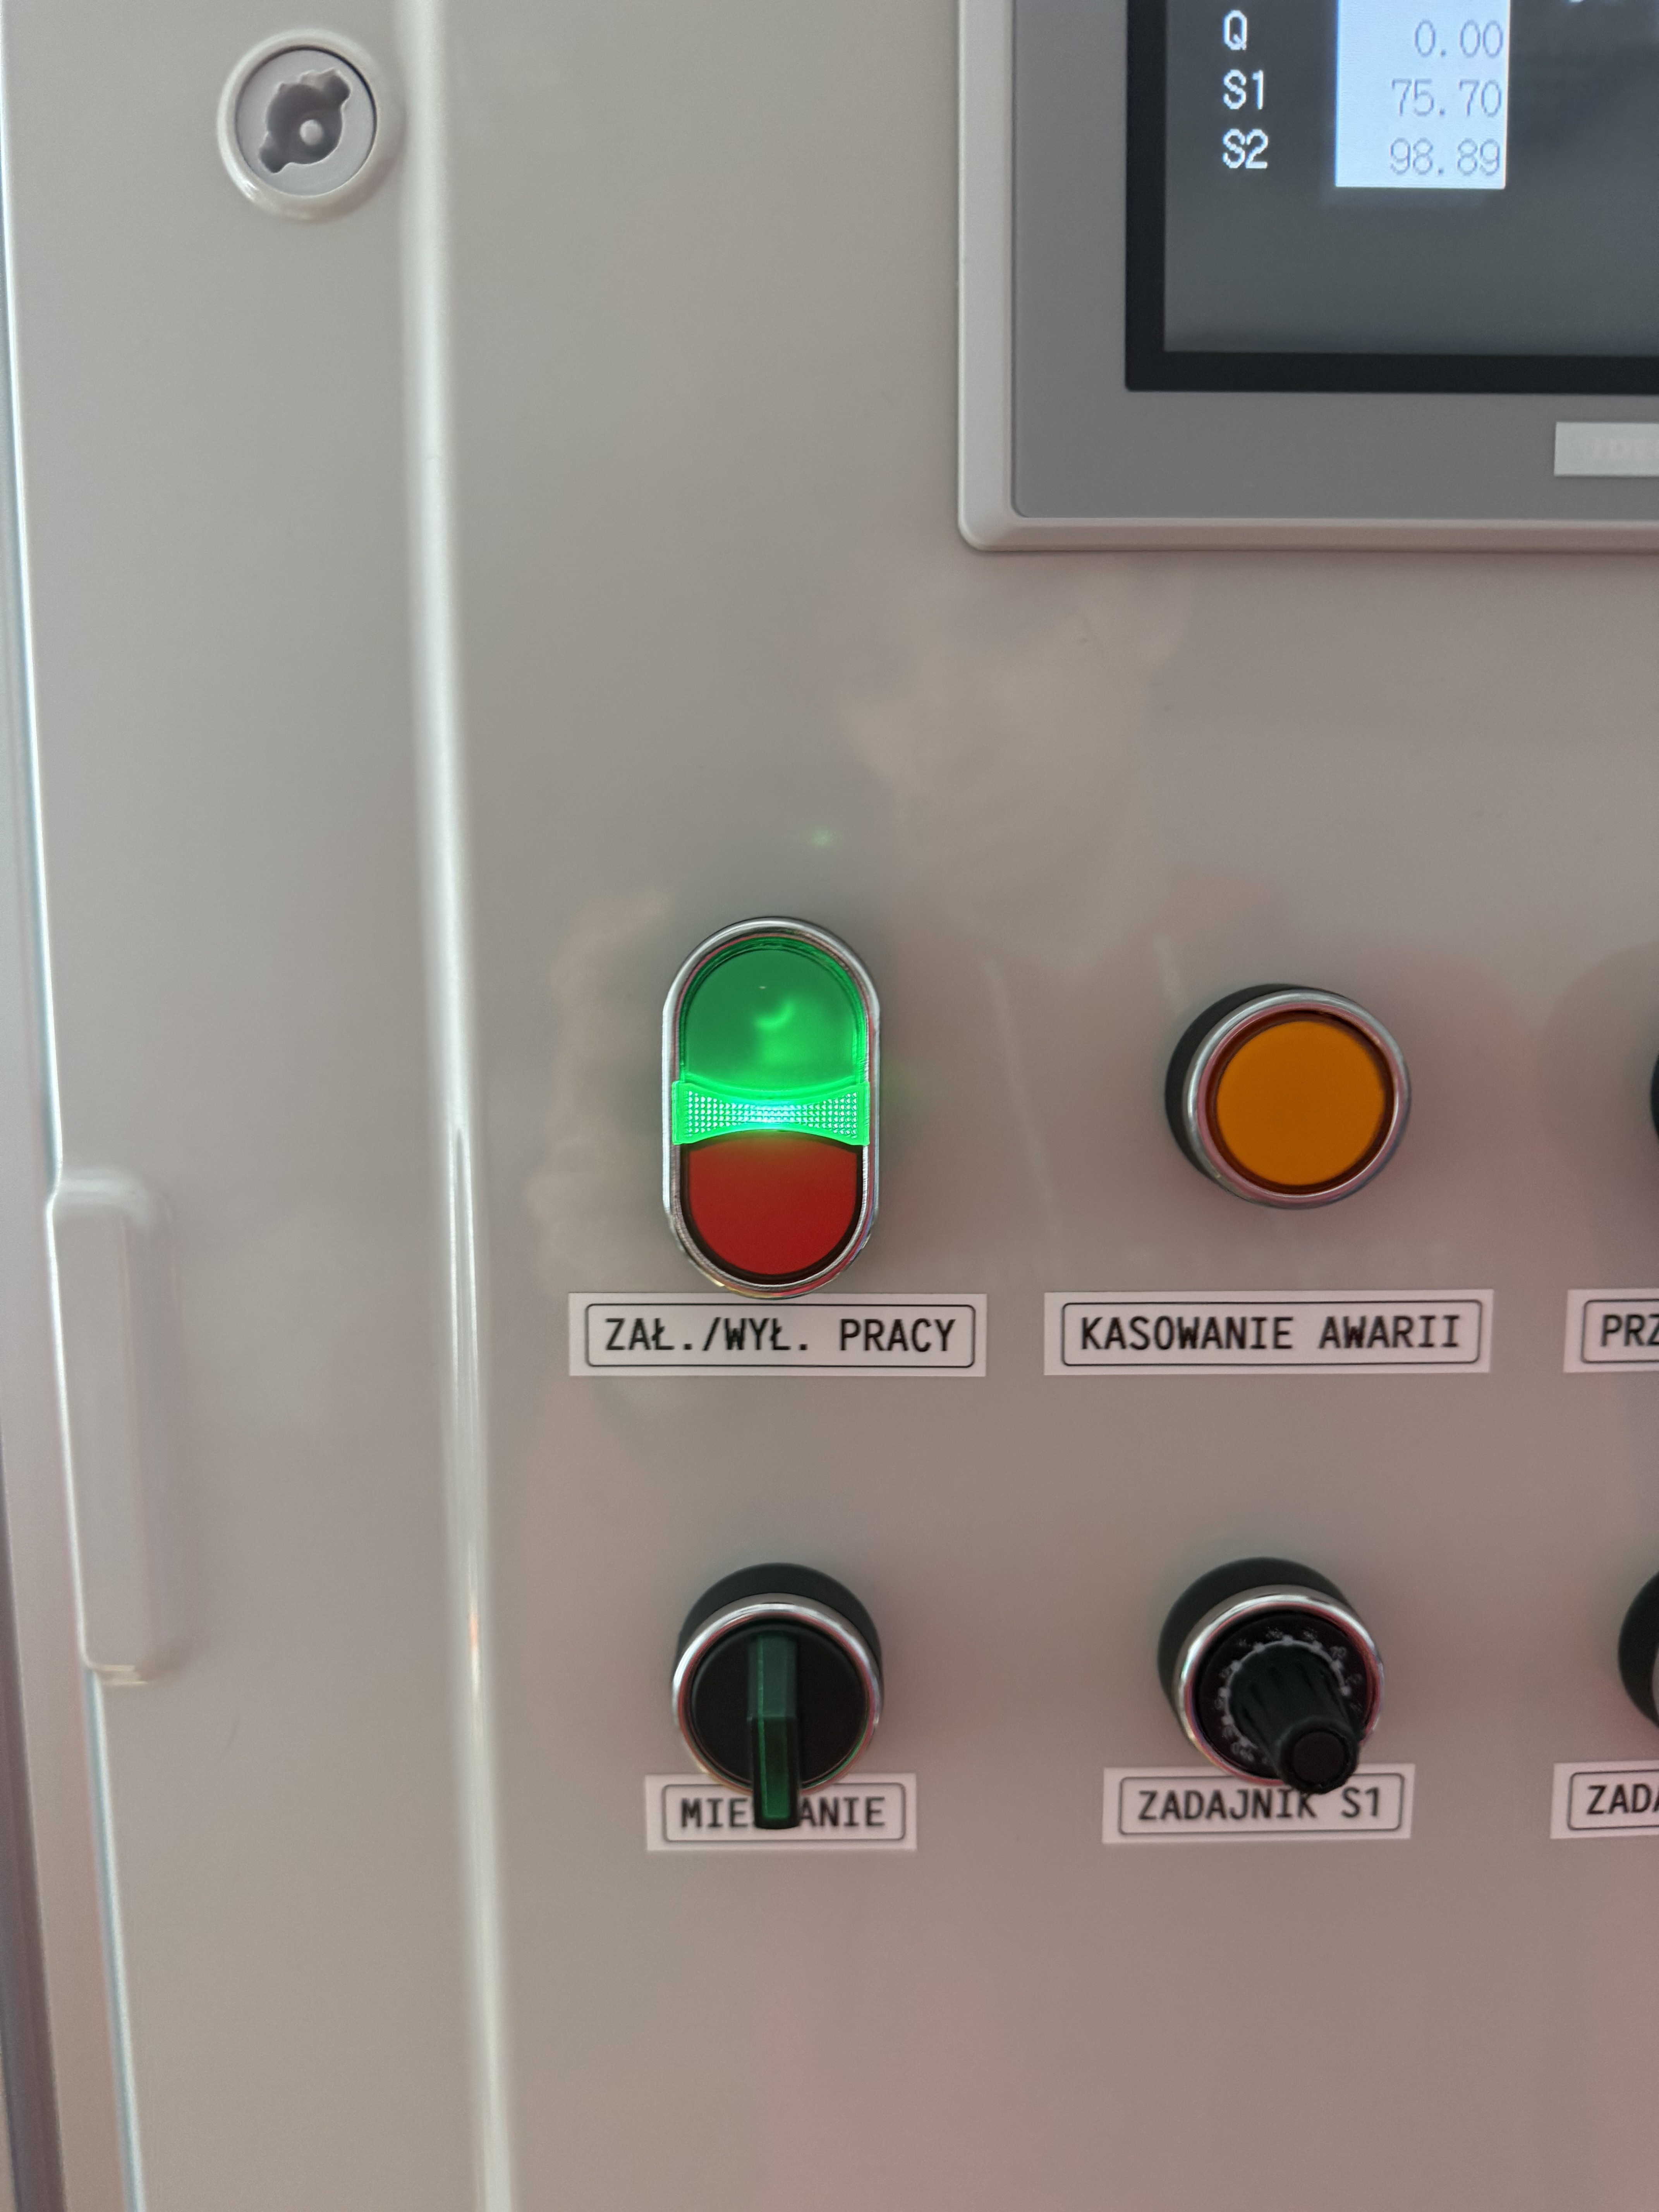
\includegraphics[width=0.5\textwidth]{media/2_1_5Kontrolki.jpeg}
    \caption{Działanie zielonej lampki}
    \label{fig:zdj10}
\end{figure}

Dodatkowo należało stworzyć drabinki które za zadanie miały:
\begin{itemize}
    \item Kontrole pompy za pomocą zmiennej \textit{I13} odpowiadającej za przełącznik na skrzynce sterowniczej.
    \item Kontrole pomarańczowej lampki, która zapala się przy dostaniu sygnału od jednej z czujek poziomu przypisanym do wartości \textit{I03} oraz \textit{I04}.
    \item Kontrole wydajności pompy za pomocą zmiennej \textit{Q10} odpowiadającego potencjometrowi na skrzynce sterowniczej.
\end{itemize}

Dodatkowo należało w zakładce \textit{Monitor/Custom} dodać zmienne procesowe \textit{D1200} oraz \textit{D1202} odpowiadającym za kontrolowanie przepustowości zaworów.

Zbudowanie takiego programu pozwala na kontrolowanie całego układu. Kod odpowiadający za logikę programu przedstawia zdjęcie \ref{fig:zdj11}.

\begin{figure}[H]
    \centering
    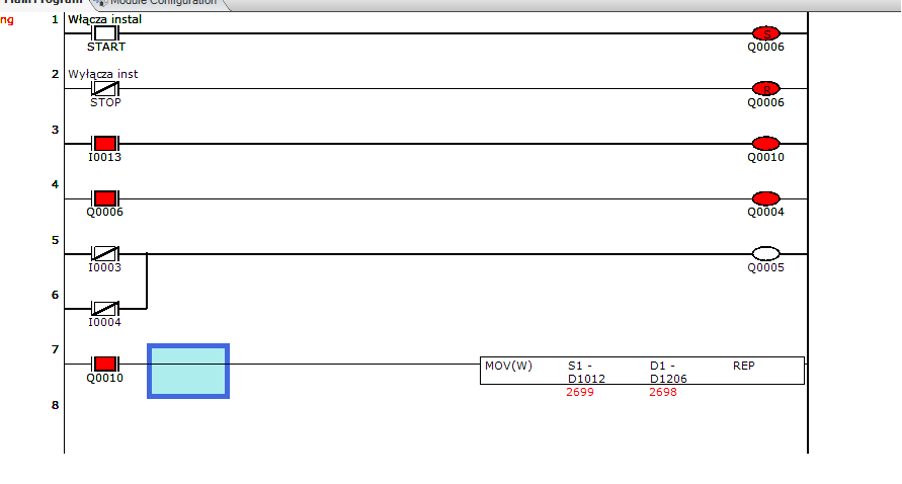
\includegraphics[width=0.5\textwidth]{media/2_2_Giga_mega_uklad.png}
    \caption{Program do kontroli stanowiska}
    \label{fig:zdj11}
\end{figure}

Na zdjęciach \ref{fig:main2} przedstawiono jak wygląda włączony układ w przypadku przepełnienia jednego z zbiorników, powodujące włączenie pomarańczowej lampki. 

\begin{figure}[H]
    \centering
        % Pod figura 1
        \subfloat[Moduł I]{    
            \centering
            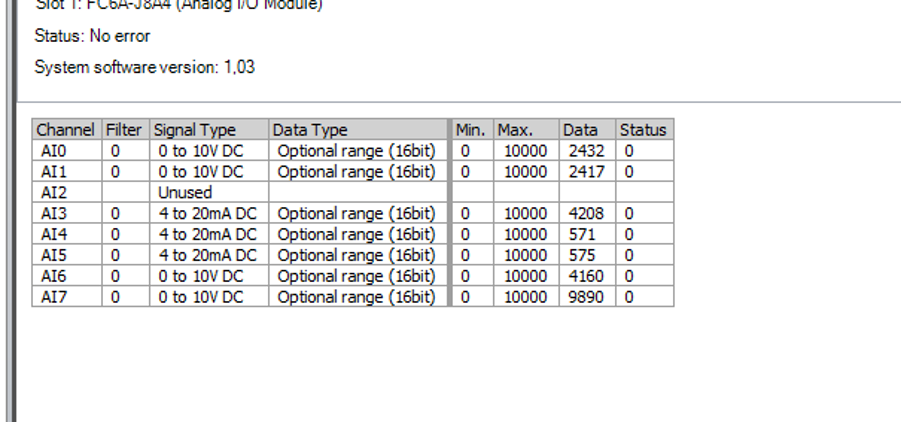
\includegraphics[width=0.45\textwidth]{media/2_4_Moduł_1_Pelne_pomerancz.png}
            \label{fig:zdj12}}
        % Pod figura 1
        \subfloat[Moduł II]{
            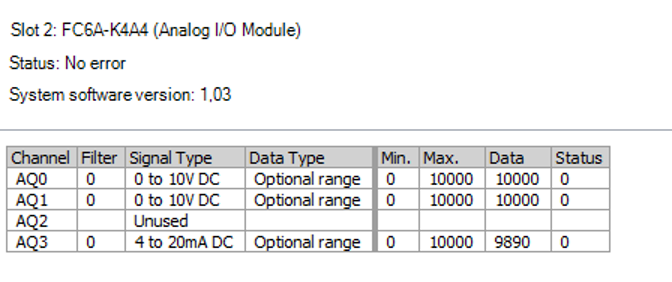
\includegraphics[width=0.45\textwidth]{media/2_3_Modul_2_zbiornik_pelny.png}        
            \label{fig:zdj13}}
    \caption{Stan awaryjny w przypadku przepełnienia zbiornika}
    \label{fig:main2}
\end{figure}

\newpage
\section{Podsumowanie}
Na zajęciach mieliśmy możliwość zapoznania się z sterownikiem PLC firmy IDEC, oraz również nauczenia się jak można zaprogramować analogowe wejścia oraz wyjścia znajdujące się w skrzynce sterowniczej.
Dzięki temu można było nauczyć się jak można skonfigurować sterownik oraz jak można go zaprogramować. Dodatkowo można było nauczyć się jak można kontrolować zmienne procesowe oraz jak można je odczytać.
Dodatkowo można było sie nauczyć jak zaprogramować sterownik aby nie wysyłał tylko informacji zero-jedynkowej ale również ciągłe, co posłużyło nam do kontroli pompy.

Całość zajęć była bardzo interesująca, ponieważ można było zobaczyć jak można wykorzystać sterownik PLC do kontroli układu. Dodatkowo można było nauczyć się jak można skonfigurować oraz zaprogramować sterownik PLC.


\end{document}
